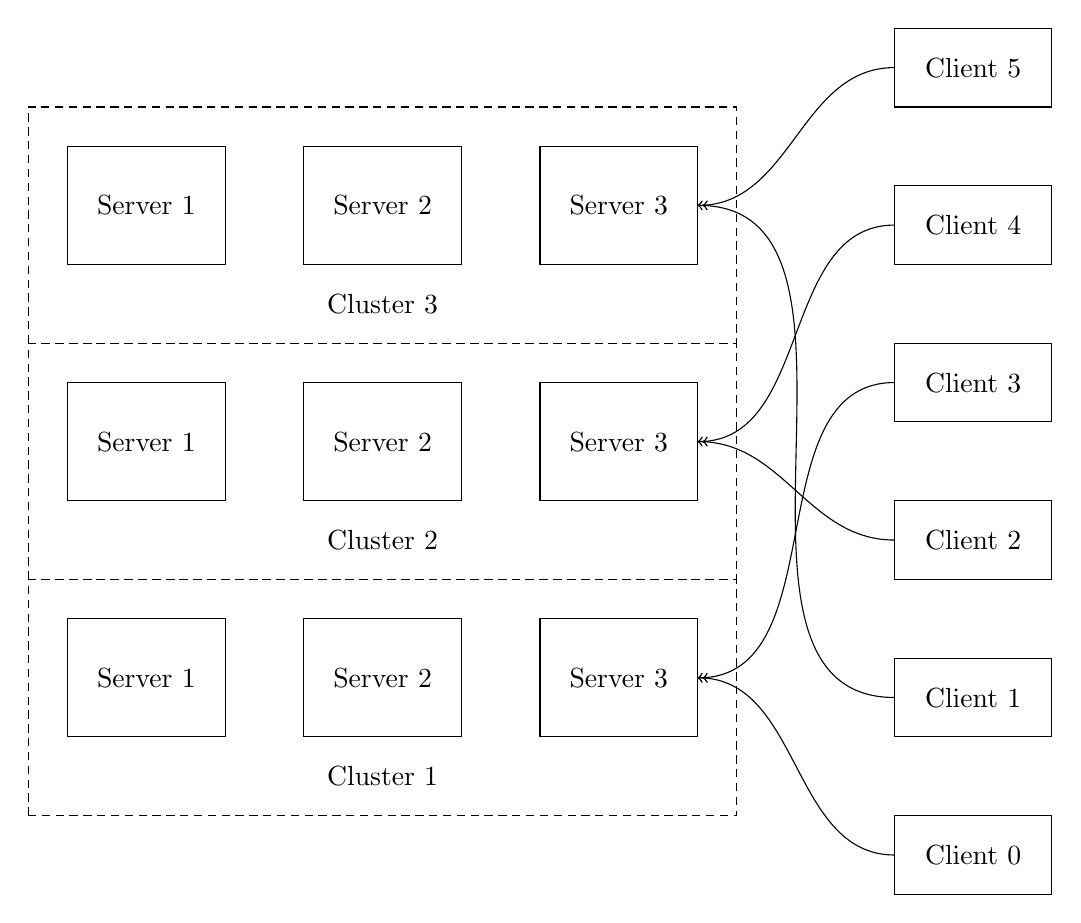
\begin{tikzpicture}
    % \draw[help lines,step=.2] (-2,-2) grid (10,4);
    \draw (0,0) rectangle(2,1.5);
    \node at (1,0.75) {Server 1};
    \draw (3,0) rectangle(5,1.5);
    \node at (4,0.75) {Server 2};
    \draw (6,0) rectangle(8,1.5);
    \node at (7,0.75) {Server 3};
    \draw[densely dashed] (-0.5,-1.0) rectangle (8.5,2);
    \node at (4.0, -0.5){Cluster 1};
    
    
    \draw (0,3) rectangle(2,4.5);
    \node at (1,3.75) {Server 1};
    \draw (3,3) rectangle(5,4.5);
    \node at (4,3.75) {Server 2};
    \draw (6,3) rectangle(8,4.5);
    \node at (7,3.75) {Server 3};
    \draw[densely dashed] (-0.5,2.0) rectangle (8.5,5);
    \node at (4.0, 2.5){Cluster 2};
    
    \draw (0,6) rectangle(2,7.5);
    \node at (1,6.75) {Server 1};
    \draw (3,6) rectangle(5,7.5);
    \node at (4,6.75) {Server 2};
    \draw (6,6) rectangle(8,7.5);
    \node at (7,6.75) {Server 3};
    \draw[densely dashed] (-0.5,5.0) rectangle (8.5,8);
    \node at (4.0, 5.5){Cluster 3};
    
    \foreach \y in {0,1,2,3,4,5}
    {
        \draw (10.5,\y*2-2) rectangle(12.5,\y*2-1);
        \node at (11.5,\y*2-1.5) {Client \y};
    }
    
    \draw[->>, thin] (10.5,-1.5)  to [out=180,in=0,looseness=1] (8,0.75);
    \draw[->>, thin] (10.5,0.5)  to [out=180,in=0,looseness=1] (8,6.75);
    \draw[->>, thin] (10.5,2.5)  to [out=180,in=0,looseness=1] (8,3.75);
    \draw[->>, thin] (10.5,4.5)  to [out=180,in=0,looseness=1] (8,0.75);
    \draw[->>, thin] (10.5,6.5)  to [out=180,in=0,looseness=1] (8,3.75);
    \draw[->>, thin] (10.5,8.5)  to [out=180,in=0,looseness=1] (8,6.75);

\end{tikzpicture}
